\section{Requirement analysis}
\label{sec:req}

Bob (made-up client for the project) consumes alcohol and can feel its effects in his bloodstream, but does not know when to stop or if he is on a safe-to-drink amount of alcohol. Bob requires a simple interactive tool that he can use on the go to check his alcohol level without being too specific about the details.\\
  
Bob should not be the only one to access this tool, so it should be available on the Web. He does not need the tool to store informations about previous alcohol level calculations, he just wants it to dynamically calculate his current alcohol level. He also wants to know how long it is going to take for his body to remove all this alcohol, for example because he absolutely needs to drive tomorrow morning to go to work. So when he uses Beerculator, Bob would like to be able to perform all the actions described in {\sc figure}~\ref{fig:useCase}.\\

\begin{figure}[H]
\centering
   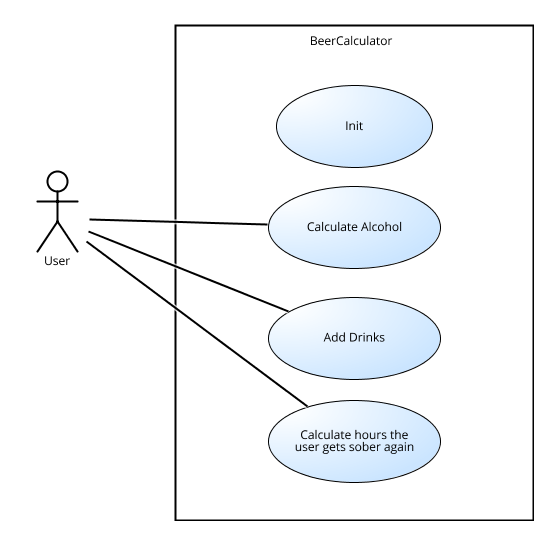
\includegraphics[scale=0.8]{./figures/UseCase.png}
   \caption{User case diagram for Beerculator}
   \label{fig:useCase}
\end{figure}

In order to perform the calculations, Beerculator needs to know a few informations about Bob: his gender, his weight, the amount of alcohol he has consumed, and also the time when the drinking started. This will be detailed in {\sc section}~\ref{sec:spec}.